%&format -translate-file pdf
\documentclass{article}
\usepackage{graphicx}
\usepackage{listings}
\lstset{basicstyle=\ttfamily\tiny}
\title{Project 4}
\author{RT Hatfield}
\date{3 November 2016}
\begin{document}
\maketitle
\begin{itemize}
    \item Here is my code.  The comments explain the complexity:
    \begin{lstlisting}
public ResultTable.Result Align_And_Extract(GeneSequence sequenceA, GeneSequence sequenceB, bool banded)
{
    
    int score;                                                       // place your computed alignment score here
    string[] alignment = new string[2];                              // place your two computed alignments here



    int X_dim = sequenceA.Sequence.Length > MaxCharactersToAlign ? MaxCharactersToAlign : sequenceA.Sequence.Length;
    int Y_dim = sequenceB.Sequence.Length > MaxCharactersToAlign ? MaxCharactersToAlign : sequenceB.Sequence.Length;


    int[,,] NW_Result;

    if (banded)
    {
        NW_Result = NW_Banded(sequenceA, sequenceB, X_dim, Y_dim);
    }
    else
    {
        NW_Result = NW_Unbanded(sequenceA, sequenceB, X_dim, Y_dim);
    }
    string[] NW_Alignment = NW_Extract(NW_Result, X_dim, Y_dim, sequenceA, sequenceB);

    // ********* these are placeholder assignments that you'll replace with your code  *******
    score = NW_Result[X_dim, Y_dim, 0];                                                
    alignment[0] = NW_Alignment[0];
    alignment[1] = NW_Alignment[1];
    // ***************************************************************************************

    ResultTable.Result result = new ResultTable.Result();
    result.Update(score,alignment[0],alignment[1]);                  // bundling your results into the right object type 
    return(result);
}

private int[,,] NW_Unbanded(GeneSequence sequenceA, GeneSequence sequenceB, int X_dim, int Y_dim)
{
    char[] A = sequenceA.Sequence.ToCharArray();
    char[] B = sequenceB.Sequence.ToCharArray();

    int[,,] result = new int[X_dim + 1, Y_dim + 1, 2];

    // we now have a 3-D array.  
    //  result[x][y][0] is the score
    //  result[x][y][1] is the alignment backpointer
    //      1 is up, 3 is left, 4 is diagonal
    //      (think Cartesian plane quadrants)
// Since this is the only data structure in use, and since it is only variable in size in 
//	the two dimensions of the inputs, it ends up being O(mn) space complexity.  It can be 
//	thought of as two identical rectangles in memory, the size of each of which is proportional 
//	to the product of the lengths of the inputs.

    // now, populate the first row and column:	linear time
    result[0, 0, 0] = 0;
    result[0, 0, 1] = 4;
    for (int i = 1; i <= X_dim; i++)
    {
        result[i, 0, 0] = result[i - 1, 0, 0] + INDEL_SCORE;
        result[i, 0, 1] = LEFT;
    }
    for (int i = 1; i <= Y_dim; i++)
    {
        result[0, i, 0] = result[0, i - 1, 0] + INDEL_SCORE;
        result[0, i, 1] = UP;
    }

    // now, begin the Needleman-Wunsch algo proper:
    for (int x = 1; x <= X_dim; x++)
    {
        for (int y = 1; y <= Y_dim; y++)	// O(xy) = O(mn).  The interior is constant time.
        {
            int end_score;
            int end_align;

            end_score = result[x - 1, y, 0] + INDEL_SCORE;
            end_align = LEFT;
            if (end_score > result[x, y - 1, 0] + INDEL_SCORE)
            {
                end_score = result[x, y - 1, 0] + INDEL_SCORE;
                end_align = UP;
            }
            // not an else, must try all options
            if (A[x - 1] == B[y - 1]) 
            {
                // check match score
                if (end_score > result[x - 1, y - 1, 0] + MATCH_SCORE)
                {
                    end_score = result[x - 1, y - 1, 0] + MATCH_SCORE;
                    end_align = DIAG;
                }
            }
            else
            {
                //check substitution score
                if (end_score > result[x - 1, y - 1, 0] + SUB_SCORE)
                {
                    end_score = result[x - 1, y - 1, 0] + SUB_SCORE;
                    end_align = DIAG;
                }
            }

            result[x, y, 0] = end_score;
            result[x, y, 1] = end_align;
        }
    }

    return result;
}

private int[,,] NW_Banded(GeneSequence sequenceA, GeneSequence sequenceB, int X_dim, int Y_dim)
{
    char[] A = sequenceA.Sequence.ToCharArray();
    char[] B = sequenceB.Sequence.ToCharArray();

    int[,,] result = new int[X_dim + 1, Y_dim + 1, 2];

    // we now have a 3-D array.  
    //  result[x][y][0] is the score
    //  result[x][y][1] is the alignment backpointer
    //      1 is up, 3 is left, 4 is diagonal
    //      (think Cartesian plane quadrants)
// Again, O(mn) space.  Same data structure, same space complexity.

    // now, populate the table with max_value, as well as INDEL vals in first row and col
    for (int x = 0; x <= X_dim; x++)	// this is O(mn) time, but the interior is very fast
    {
        for (int y = 0; y <= Y_dim; y++)
        {
            result[x, y, 0] = Int32.MaxValue - 100;
        }
    }
    result[0, 0, 0] = 0;
    result[0, 0, 1] = 4;
    for (int i = 1; i <= 3; i++)	// these are linear time
    {
        result[i, 0, 0] = result[i - 1, 0, 0] + INDEL_SCORE;
        result[i, 0, 1] = LEFT;
    }
    for (int i = 1; i <= 3; i++)
    {
        result[0, i, 0] = result[0, i - 1, 0] + INDEL_SCORE;
        result[0, i, 1] = UP;
    }

    // since Needleman-Wunsch can't be banded with strings differing more than the bandwidth in length
    // just skip the whole thing to save time then
    if (X_dim - Y_dim > 3 || X_dim - Y_dim < -3)
    {
        return result;
    }

    // now, begin the Needleman-Wunsch algo proper: 
// The outer loop is linear in the size of one input.  
//	The inner loop is essentially constant time.  The interior is constant.
//  However, you have to check all of both strings, so it ends up being
//	linear in the larger of the two inputs, or O(m + n).
    for (int y = 1; y <= Y_dim; y++)
    {
        for (int x = (y - 3 < 1 ? 1 : y - 3); x <= y + 3 && x <= X_dim; x++)
        {

            int end_score;
            int end_align;

            end_score = result[x - 1, y, 0] + INDEL_SCORE;
            end_align = LEFT;
            if (end_score > result[x, y - 1, 0] + INDEL_SCORE)
            {
                end_score = result[x, y - 1, 0] + INDEL_SCORE;
                end_align = UP;
            }
            // not an else, must try all options
            if (A[x - 1] == B[y - 1])
            {
                // check match score
                if (end_score > result[x - 1, y - 1, 0] + MATCH_SCORE)
                {
                    end_score = result[x - 1, y - 1, 0] + MATCH_SCORE;
                    end_align = DIAG;
                }
            }
            else
            {
                //check substitution score
                if (end_score > result[x - 1, y - 1, 0] + SUB_SCORE)
                {
                    end_score = result[x - 1, y - 1, 0] + SUB_SCORE;
                    end_align = DIAG;
                }
            }

            result[x, y, 0] = end_score;
            result[x, y, 1] = end_align;
        }
    }

    return result;
}

private string[] NW_Extract(int[,,] table, int X_dim, int Y_dim, GeneSequence sequenceA, GeneSequence sequenceB)
{
    StringBuilder A_build = new StringBuilder();
    StringBuilder B_build = new StringBuilder();

    if (table[X_dim, Y_dim, 0] == Int32.MaxValue - 100)  // in practice, this may amortize a large number of strings
    {
        return new String[] { "No Alignment Possible", "No Alignment Possible" };
    }

    string A_temp = sequenceA.Sequence;
    string B_temp = sequenceB.Sequence;

    char[] A = A_temp.Insert(0, "-").ToCharArray();
    char[] B = B_temp.Insert(0, "-").ToCharArray();

    int x = X_dim;
    int y = Y_dim;

    while (x > -1 && y > -1)	// This loop will iterate at most m+n times
    {
        if (x == 0 && y == 0)
        {
            // we kinda designed around this but let's just quit to be safe
            break;
        }

        if (table[x, y, 1] == DIAG)
        {
            // just add each character to the outputs
            A_build.Insert(0, A[x]);
            B_build.Insert(0, B[y]);
            // now climb diagonally
            x--;
            y--;
        }
        else if (table[x, y, 1] == UP)
        {
            // an indel.  
            A_build.Insert(0, '-');
            B_build.Insert(0, B[y]);
            y--;
        }
        else if (table[x, y, 1] == LEFT)
        {
            // an indel.  
            A_build.Insert(0, A[x]);
            B_build.Insert(0, '-');
            x--;
        }
    }


    return new String[] {A_build.ToString(), B_build.ToString()} ;
}
\end{lstlisting}
    \item I built my code around a three-dimensional array.  The array was $m\times n\times 2$ in size.
    The third dimension contains only two planes, which each correspond to the dynamic programming table.
    The zeroth plane contains the scores.  The first plane contains enumerated ints which act as backpointers.  "Up" to indicate that the cell above is referenced, "Diag" to indicate that the upper-left 
    cell is referenced, etc.  I used a standard Needleman-Wunsch strategy for the unrestricted algorithm.
    I simply iterated through the whole table, minimizing the score for each cell based on its neighbors,
    keeping track of which neighbor won with backpointers in the table.  For the banded algorithm, I first
    prepopulated the table with egregiously large values, such that no "empty" cell could accidentally
    become a parent of a good cell.  Then I iterated through the Y-dimension of the table, only iterating 
    through a subset of the cells on that row.  I bounded my X-coordinate by $y\pm 3$.  I scored each cell
    and memoized the scores and path in the same way as for the normal algorithm.
    
    For extracting the correct sequence, I started at the lower-right corner of the table, and read the 
    backpointers in each cell of the first plane to either select the corresponding letters from both 
    strings, or to insert an indel and traverse either right or left appropriately.  I did this continuously
    until I exited the table, having reconstituted the entire alignment of both strings.
    \item \begin{lstlisting}
gattgcgagcgatttgcgtgcgtgcatcccgcttc-actg--at-ctcttgttagatcttttcataatctaaactttataaaaacatccactccctgta-
-ataa-gagtgattggcgtccgtacgtaccctttctactctcaaactcttgttagtttaaatc-taatctaaactttataaa--cggc-acttcctgtgt
    \end{lstlisting}
    \item See Figure 1 and Figure 2.
    \begin{figure}[p]
        \centering
        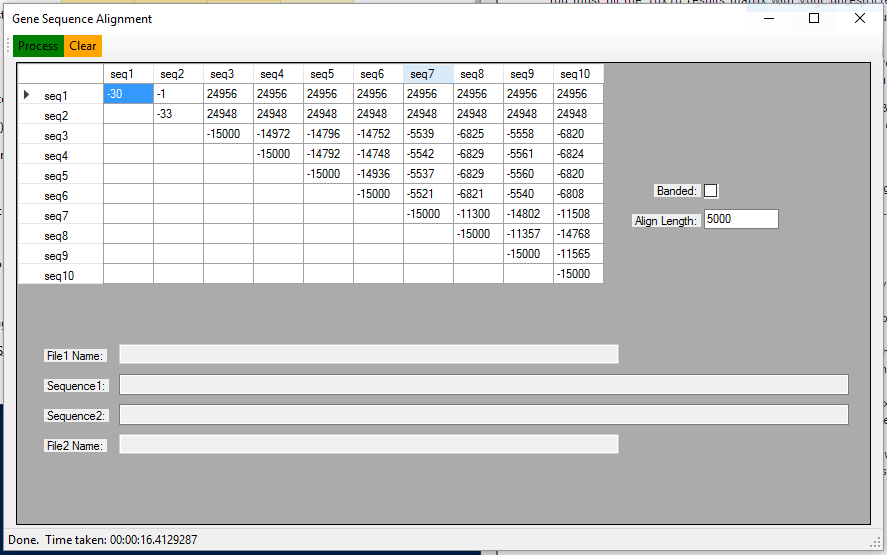
\includegraphics[resolution=72, width=\textwidth]{Capture}
        \caption{unbanded}
    \end{figure}
        \begin{figure}[p]
        \centering
        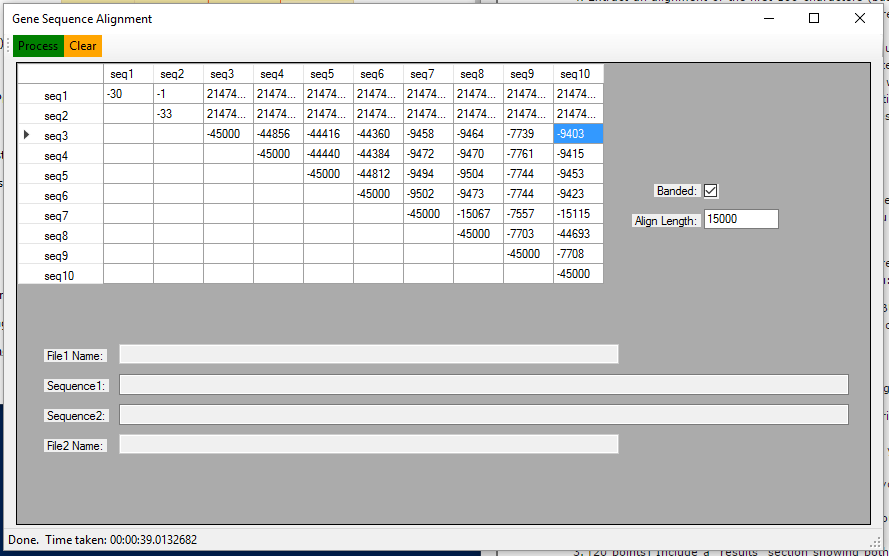
\includegraphics[resolution=72, width=\textwidth]{Capture2}
        \caption{banded}
    \end{figure}
\end{itemize}
\end{document}
